\documentclass{article}


%%%%%%%%%%%%%%%%%%%%%%%%
%%%%%%%%%%%%%%%%%%%%%%%%
%%%%%%Packages
%%%%%%%%%%%%%%%%%%%%%%%%
%%%%%%%%%%%%%%%%%%%%%%%%

\usepackage{amsthm}
\usepackage{amsmath}
\usepackage{amssymb}
\usepackage[margin=1in]{geometry}
\usepackage{enumerate}
\usepackage{color}
\usepackage{graphicx}



%%%%%%%%%%%%%%%%%%%%%%%%
%%%%%%%%%%%%%%%%%%%%%%%%
%%%%%%amsthm settings
%%%%%%%%%%%%%%%%%%%%%%%%
%%%%%%%%%%%%%%%%%%%%%%%%

\theoremstyle{definition}
\newtheorem{problem}{Theorem}
\newtheorem{claim}{Claim}
\newtheorem{definition}{Definition}

%%%%%%%%%%%%%%%%%%%%%%%%
%%%%%%%%%%%%%%%%%%%%%%%%
%%%%%%Custom commands: mathbb
%%%%%%%%%%%%%%%%%%%%%%%%
%%%%%%%%%%%%%%%%%%%%%%%%

\newcommand{\A}{\mathbb A}
\newcommand{\C}{\mathbb{C}}
\newcommand{\D}{\mathbb{D}}
\newcommand{\E}{\mathbb{E}}
\newcommand{\F}{\mathbb{F}}
\newcommand{\N}{\mathbb{N}}
\renewcommand{\P}{\mathbb{P}}
\newcommand{\R}{\mathbb{R}}
\newcommand{\X}{\mathbb{X}}
\newcommand{\Z}{\mathbb{Z}}
\newcommand{\Q}{\mathbb{Q}}

%%%%%%%%%%%%%%%%%%%%%%%%
%%%%%%%%%%%%%%%%%%%%%%%%
%%%%%%Custom commands: greek
%%%%%%%%%%%%%%%%%%%%%%%%
%%%%%%%%%%%%%%%%%%%%%%%%

\renewcommand{\a}{\alpha}
\renewcommand{\b}{\beta}
\newcommand{\g}{\gamma}
\renewcommand{\d}{\delta}
\newcommand{\e}{\epsilon}
\renewcommand{\l}{\lambda}

\usepackage[utf8]{inputenc}

\title{Homework 2}
\author{Sean Eva}
\date{Math 4320}

\begin{document}

\maketitle

\begin{enumerate}
    \item [[\phantom{-}1]]
    
    \begin{enumerate}
        \item 
        
        Not a domain
        \begin{figure}[h]
            \centering
            \includegraphics[width=0.4\textwidth]{1a.png}
        \end{figure} 
        
        \item
        
        A domain
        \begin{figure}[h]
            \centering
            \includegraphics[width=0.4\textwidth]{1b.png}
        \end{figure}
        \\\\\\\\\\\\
        
        \item
        
        A domain
        \begin{figure}[h]
            \centering
            \includegraphics[width=0.4\textwidth]{1c.png}
        \end{figure} 
        
        \item
        
        Not a domain
        \begin{figure}[h]
            \centering
            \includegraphics[width=0.4\textwidth]{1d.png}
        \end{figure}
        \\\\\\\\\\\\\\\\\\\\\\\\\\
        
        \item
        
        Not a domain
        \begin{figure}[h]
            \centering
            \includegraphics[width=0.4\textwidth]{1e.jpg}
        \end{figure} 
        
        \item
        
        Not a domain
        \begin{figure}[h]
            \centering
            \includegraphics[width=0.4\textwidth]{1f.png}
        \end{figure} 
        
    \end{enumerate}
    
    \item [[\phantom{-}2]]
    
    The only set from Exercise 1 that is neither open nor closed is part e $0\leq arg(z) \leq \pi/4 (z\neq 0)$ because there is no $\epsilon > 0$ that the area would be encompassed in for all values of $r.$
    
    \item [[\phantom{-}5]]
    
    \begin{proof}
    Let the two sets be as they are in the problem statement. We can consider these two sets as open balls where one is centered at $x = 0$ and $x = 2$ with radius $1.$ Let us then say that these two sets are jointed, where we could define $z_0$ as being within both sets. Then we have $x = |z_0 - (z_0 - 2)| \leq |z_0| + |z_0 - 2| < 2$ which is a contradiction since it states that $2 < 2$ which is false. Therefore, we know that these two sets are disjointed. Since these two sets are open and disjointed, it follows then that they are disconnected.
    \end{proof}
    
    \item [[\phantom{-}1]]
    
    $f(z) = (\frac{z + \bar{z}}{2})^2 - (\frac{z - \bar{z}}{2i})^2 - 2(\frac{z - \bar{z}}{2i}) + i(2(\frac{z + \bar{z}}{2}) - 2(\frac{z + \bar{z}}{2})(\frac{z - \bar{z}}{2i})) = \frac{z^2 + \bar{z}^2 + 2z\bar{z}}{4} - \frac{z^2 + \bar{z}^2 - 2z\bar{z}}{-4} - \frac{z - \bar{z}}{i} + i(z + \bar{z}) - \frac{z^2 - \bar{z}^2}{2} = \bar{z}^2 + 2iz$. Therefore, we have that $f(z) = \bar{z}^2 + 2iz$ as desired.
    
    \item [[\phantom{-}6]]
    
    Let us take the given transformation of $\omega = z^2 = (x + iy)^2 = (x^2 - y^2) + 2ixy$ thus making $u = x^2 - y^2$ and $v = 2xy$. Then for the first hyperbola, we know that $c_1 = (x^2 - y^2)$ so then we know that $\omega = c_1 + iv$. So it is a straight line as:
    \begin{figure}[h]
            \centering
            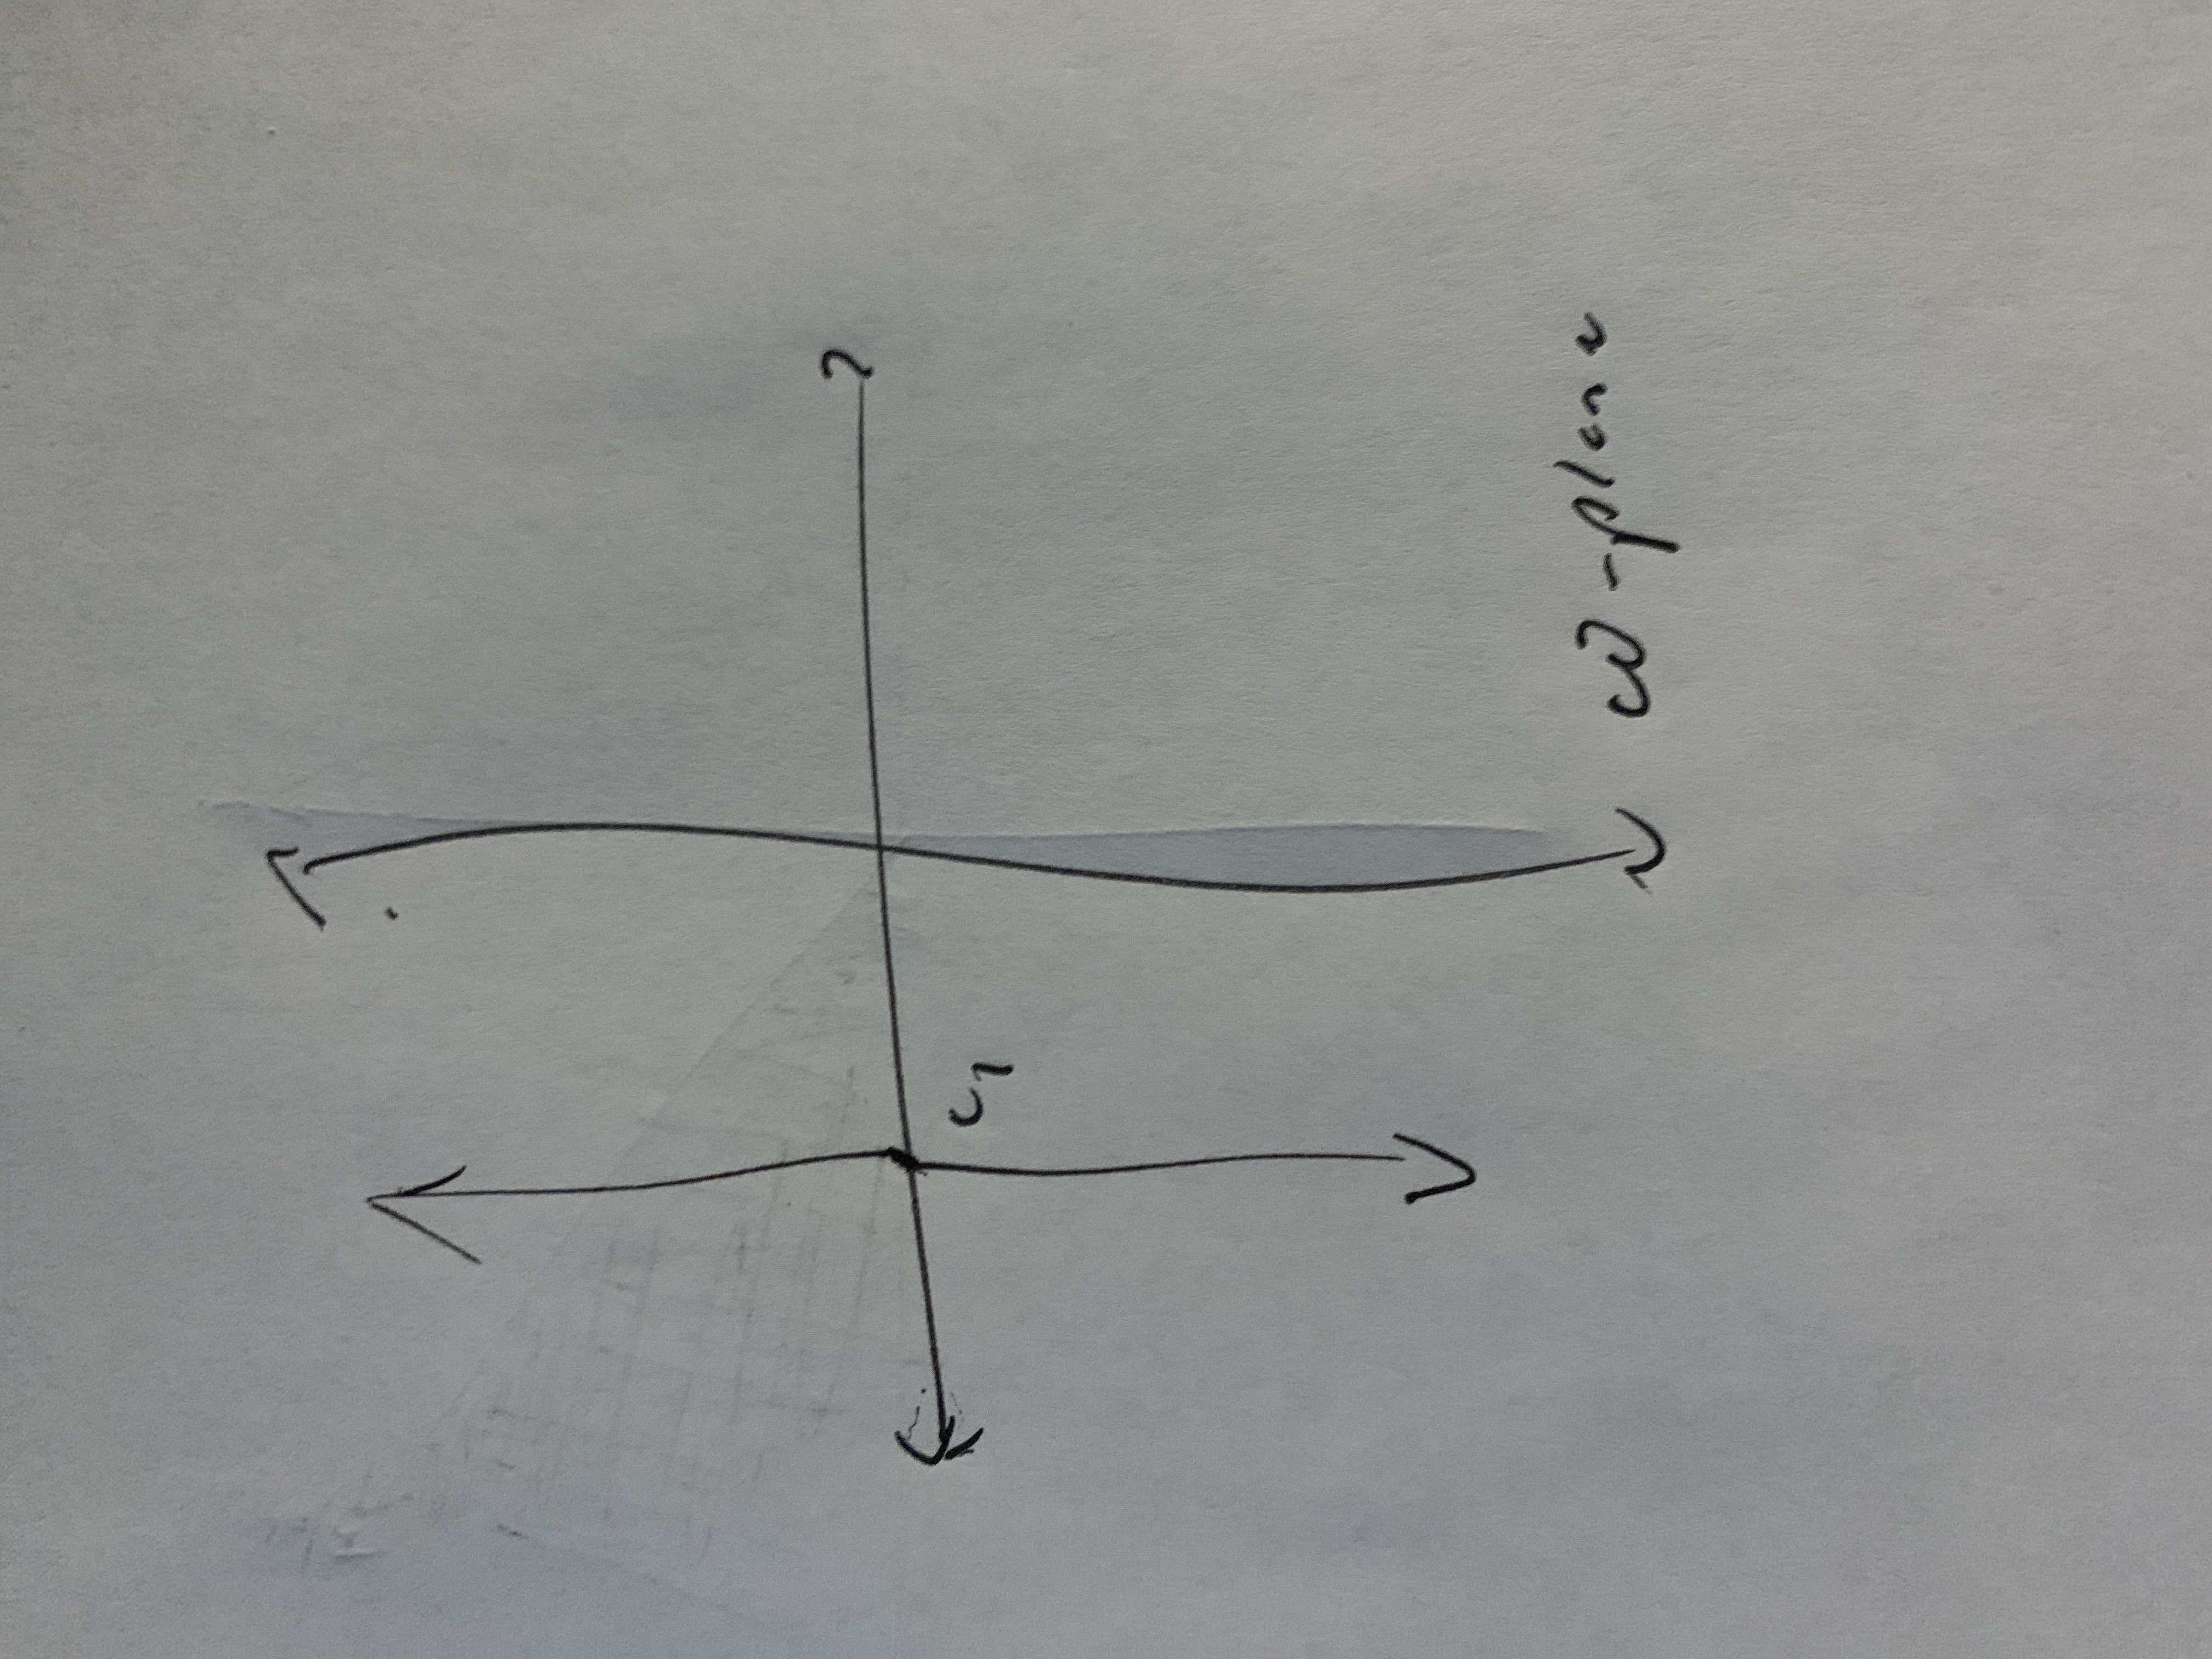
\includegraphics[width=0.4\textwidth]{6a.jpg}
    \end{figure}
    \\
    For the second hyperbola, we have that $c_2 = 2xy$ and with the same transofmration wer have that $\omega = u + ic_2$ which would again make the image a straight like as: 
    \begin{figure}[h]
            \centering
            \includegraphics[width=0.4\textwidth]{6b.jpg}
    \end{figure}
    
\end{enumerate}

\end{document}
